\section{Client Application}
\label{design:client-application}

This section discusses the~design aspects of the~client application of the\linebreak{}designed game.
It discusses platforms that can be used and their limitations and benefits.
Then there is a~discussion on different options of frameworks to use according to platform specifications with extra pieces of information about the~selected framework and how it works.
Also, the~client architecture is described and designed according to previous chapters. 
And last but not least, the~state management selection and options discussion is done.

\subsection{Platforms}

The~designed game targets especially web and desktop platforms.
One of the~non-functional requirements is that it should be possible to extend the\linebreak{}game to other platforms, like mobiles.
The~web and desktop platforms are pretty similar.
They are both used on computers and use similar resolutions and workflow.
On the~other hand, the~mobile platform uses entirely different resolutions, and its users use their hands to control the~screen's content.
Mobiles also often have slow internet connections, and the~design of the~game for mobile in general and the~extension of the~game to mobiles in the~future should count with this.

For the~design of the~game \myAppName{}, the~development of an~application for the~web platform and the~desktop platform, targeting the~Windows operating system, will be considered.

\subsubsection{Cross-Origin Resource Sharing}

\begin{figure}
    \centering
    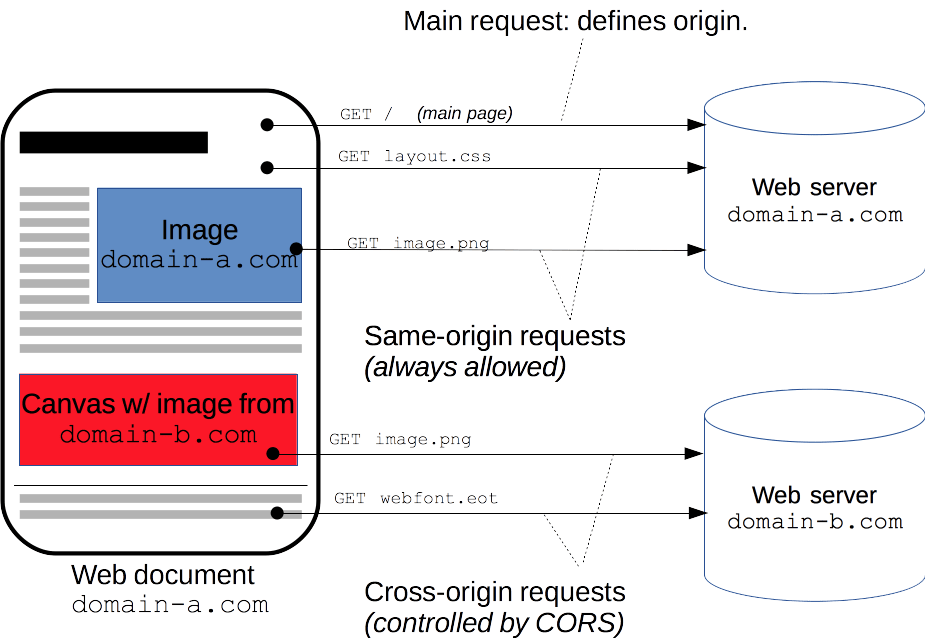
\includegraphics[width=1\linewidth]{assets/design/cors.png}
    \caption{The~CORS Mechanism~\cite{a2022_crossorigin}}
    \label{fig:design:cors-mechanism}
\end{figure}

The~web platform also has its limitations.
Modern web browsers include mechanisms that permit loading resources only from trusted client sources for security reasons.
When a~web application initiates a~\mintinline{js}{XMLHttpRequest} or uses the~Fetch API, a~browser requires that it must follow the~same-origin policy.
This mechanism is called CORS, and it means Cross-Origin Resource Sharing.

As stated in~\cite{a2022_crossorigin}, CORS is a~mechanism that lets servers specify trusted origins using HTTP headers.
Its purpose is to protect users and their cookies and other stuff stored in the~browser specifically.
Not enforcing the~same-origin policy could be a~potential risk for applications, e.g., banks that use cookies to verify that you are who you are, and using some malicious software attackers could dry out bank accounts.
That is not an~issue on desktop and mobile because cookies are stored inside applications' storage, and other\linebreak{}applications cannot access their cookies; therefore, these data can not be stolen.
The~essential idea from this concept is that this is not the~applications' fault; it is the~browsers' fault.
Servers set the~\mintinline{text}|Access-Control-Allow-Origin| header, and if matched with the~origin, a~browser allows the~application\linebreak{}to view and process its response.

The~header format \mintinline{text}/Access-Control-Allow-Origin: <origin> | */ must be used.
It can also be set with wildcards to relax the~CORS specification.
Communication between an~application and a~server with same-origin and cross-origin requests and their responses can be seen in the~figure~\ref{fig:design:cors-mechanism}.

\subsection{Frameworks}

It is often possible to use various libraries and frameworks to develop games and applications, making it easier to build software in terms of speed and capabilities.
Many experienced developers develop and optimize frameworks and develop an~efficient and versatile set of tools that allow developers who use these frameworks to take advantage of high-level functionality that addresses low-level functions such as security, component communication, dependency, and more.

Individual frameworks have different requirements and goals.
Some focus on specific programming languages, particular platforms, cross-platform mobile application development, and cross-platform development in general, whether it's mobile, web, or desktop.

Since the~developed game needs development for the~web, desktop (especially for the~Windows platform), and the~future possibility of extension to mobile devices, choosing one of the~cross-platform frameworks is necessary.
There are not many frameworks that support easy and stable development for both the~web and the~desktop and mobile devices.
Most frameworks, as mentioned, target a~single platform.
Some frameworks focus on the~development of applications or games for mobile devices, where they are further divided into development for Android and iOS~\cite{leler_2017_whats}.
They release SDKs (Software Development Kit) to develop on mentioned platforms, allowing developers to create widgets rendered to canvas and use native services.
Of course, this way does not allow the~creation of cross-platform software because of the~specificity of developing to the~individual platform, so they will not be considered.
There are also web frameworks that focus on robust web application development, which, in contrast, has an~actual usage even on mobile devices.

\begin{figure}
    \centering
    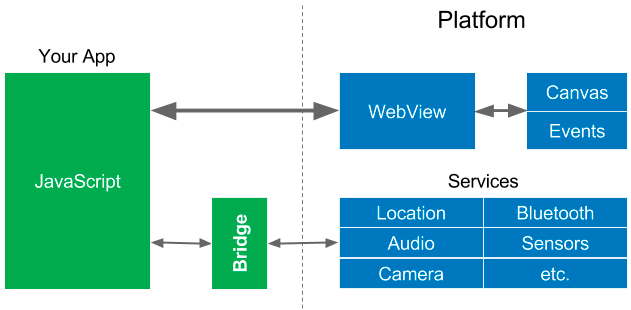
\includegraphics[width=1\linewidth]{assets/design/webview.png}
    \caption{WebView~\cite{leler_2017_whats}}
    \label{fig:design:webview}
\end{figure}

The~advantage of web frameworks over mobile ones, in terms of cross-platform development, is that thanks to technologies such as WebView and other supporting tools, it is possible to create a~mobile version of the~application.
Many cross-platform web frameworks use JavaScript with WebView, with a~design usually similar to the~figure~\ref{fig:design:webview}.
Representatives of these procedures are PhoneGap, Ionic, and other frameworks.
One of the~problems this approach has to solve is communication with device services such as cameras, Bluetooth, sensors, etc.
Therefore, the~so-called bridges, which communicate via JavaScript with native code, were most often created.

\begin{figure}
    \centering
    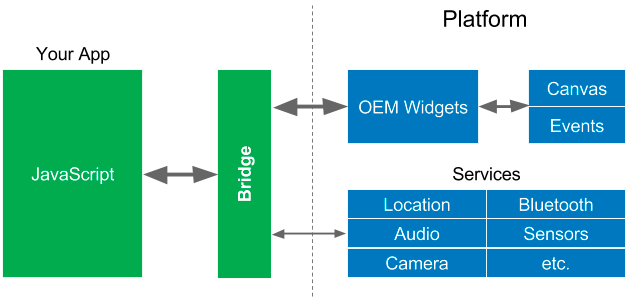
\includegraphics[width=1\linewidth]{assets/design/reactive.png}
    \caption{Reactive View~\cite{leler_2017_whats}}
    \label{fig:design:reactiveview}
\end{figure}

However, WebView does not perform well, so over time, other web frameworks have come up with different approaches.
One of these approaches is not to use WebView, but to use the~OEM (Original Equipment Manufacturer) widgets of the~platform directly for displaying~\cite{leler_2017_whats}.
One representative of this approach is React Native~\cite{a2022_react} with a design similar to the~figure~\ref{fig:design:reactiveview}.
It was created in 2015 by extending the~React web framework, both developed by Facebook~\cite{a2022_react}.
Unlike React, which uses web components, React Native uses OEM widgets.
OEM widgets are accessed from JavaScript using a~bridge that communicates with widgets and native platform services~\cite{leler_2017_whats}.
Both technologies are high-speed.
However, the~use of a~bridge causes a~communication bottleneck.
That causes a~slowdown in performance if a~lot of communication is done using the~bridge.
React Native has brought many benefits of reactive views to mobile applications.
React Native nowadays also focuses on developing for Windows, macOS, and the~web using React Native Windows, ReactNative macOS, and React Native Web~\cite{a2022_react}.
All mentioned projects use bridges to communicate with the~platform.

The~Flutter framework provides an~entirely different approach.
It has been historically developed as a~cross-platform framework for development on mobile devices.
Today, however, the~framework also supports development for the~web and desktops.
According to~\cite{leler_2017_whats}, unlike previous frameworks, which used web technologies to one degree or another, Flutter does not use JavaScript and web technologies to achieve better performance.
It uses custom widgets that are rendered to the~platform's canvas.
That also means that no matter the~operating system version, the~look and feel are always the~same because they do not rely on OEM widgets. 

\begin{figure}
    \centering
    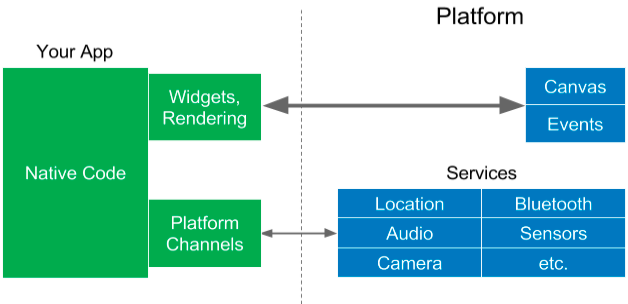
\includegraphics[width=1\linewidth]{assets/design/flutter.png}
    \caption{Flutter~\cite{leler_2017_whats}}
    \label{fig:design:flutterview}
\end{figure}

\subsubsection{Flutter}

Flutter is an~open-source framework developed by Google~\cite{a2022_flutter} that uses the Dart programming language, which allows the~ahead-of-time (AOT) compilation into native cross-platform code~\cite{leler_2017_whats}.
In addition, it allows the~just-in-time (JIT) compilation, which will enable developers to view changes almost instantly.
Compiling into native code provides many benefits, such as execution speed and performance.
\textcquote{leler_2017_whats}{The~fact that Flutter is the~only mobile SDK that provides reactive views without requiring a~JavaScript bridge should be enough to make Flutter interesting and worth trying, but there is something far more revolutionary about Flutter, and that is how it implements widgets.}
The~framework still needs to communicate with the~native platform.
The~platform channels interface is used for this purpose, as can be seen in~\ref{fig:design:flutterview}, which works on the~principle of data transfer.
The~framework encodes and decodes the~data, but overall the~whole process works faster than JavaScript bridges.

The~Dart language also contributed to the~significant improvement of Flutter 2, introducing sound null safety, which further helps Flutter type correctness and prevents null error crashes that can be caught during development~\cite{sells_2021_whats}.
This feature allows developers to use Flutter to write better and better code.
Flutter2 also introduced support for the~Add-to-app feature, enabling developers to use Flutter code inside their existing applications.

Flutter is very simple in principle.
It is designed to abstract its engine and framework from platforms, which will allow easy development on various platforms, as mentioned in~\cite{a2022_flutter_architecture}.
Platform-specific things are implemented, and the~rest of the~framework can remain unchanged, as seen in the~figure~\ref{fig:design:flutterlayers}.
No layer must interfere with the~layer below, and each part of the~system will design so that it can be replaced.
As described in~\cite{a2022_flutter_architecture}, the~embedder layer is written in the~languages appropriate for the~platform.
For Windows and Linux in C++, macOS and iOS in Objective-C or Objective-C++, and Android in Java and C++.
Embedder mediates communication with the~operating system, services, inputs, events, etc.
The~basics of Flutter are contained in the~engine layer, which is created primarily in C++.
The~engine is responsible for any rendering which uses the~Skia library.
The~Skia library is a~2D graphics library used as a~graphics engine, e.g., Google Chrome, Android, Flutter~\cite{skia_2022_skia}.
The~engine mediates the~framework using \mintinline{text}|dart:ui| libraries.
The~framework layer then provides access to a~reactive framework in the~Dart language\linebreak{}and provides a~range of widgets, layouts, gesture detectors, animation support, etc.
Developers usually use this layer.

A particular case is Flutter's web support~\cite{a2022_flutter_architecture}.
Flutter on the~web works with Dart's compiler, which compiles the~code into JavaScript.
Dart historically has a~significantly enhanced toolchain focused on compiling Dart code into JavaScript because Dart's first goal was to replace JavaScript in browsers.
Today some big applications like the~advertiser tooling for Google Ads use Dart to JavaScript compilation.
The~framework layer, written in Dart, will compile into JavaScript.
However, the~engine layer is written in C/C++; therefore, this layer cannot be used on the~web.
Similarly, it cannot use the~embedder layer to render as it is designed to run with the~operating system.
Flutter on the~web uses a~reimplemented version of the~engine above the~standard browser APIs.
This unique browser layer currently has two strategies to render.
\linebreak
It can use HTML mode to render HTML, CSS, Canvas, and SVG.
Or it can use WebGL mode, which uses CanvasKit, a~particular version of Skia library compiled to WebAssembly.
The~layers used in the~web version of Flutter can be seen in the~figure~\ref{fig:design:flutterweb}.

\begin{figure}
    \centering
    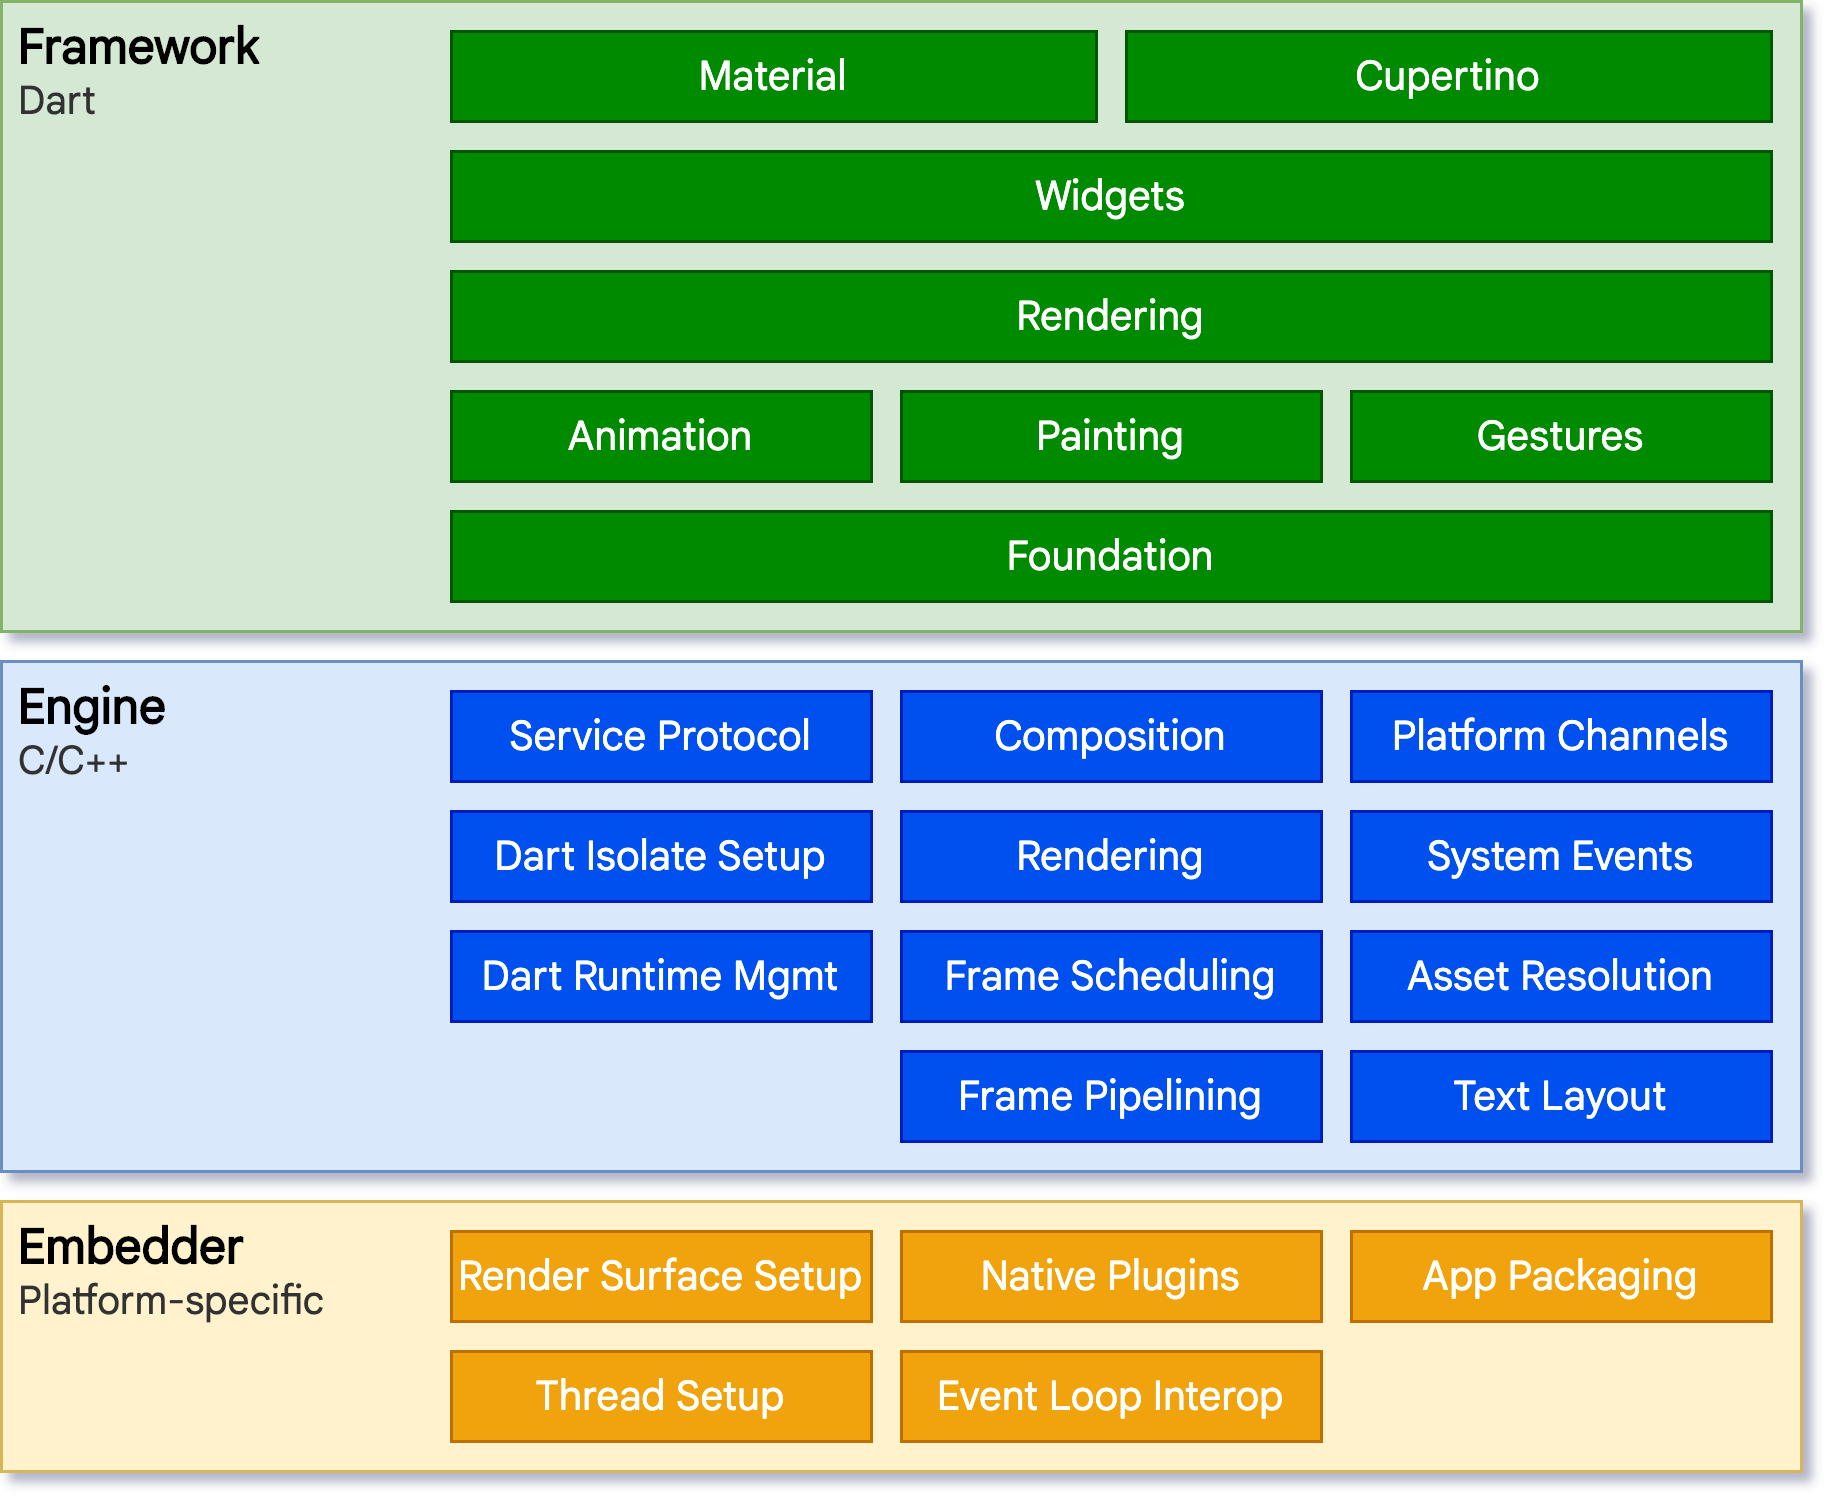
\includegraphics[width=1\linewidth]{assets/design/flutterlayers.png}
    \caption{Flutter's Architectural Layers~\cite{a2022_flutter_architecture}}
    \label{fig:design:flutterlayers}
\end{figure}

\begin{figure}
    \centering
    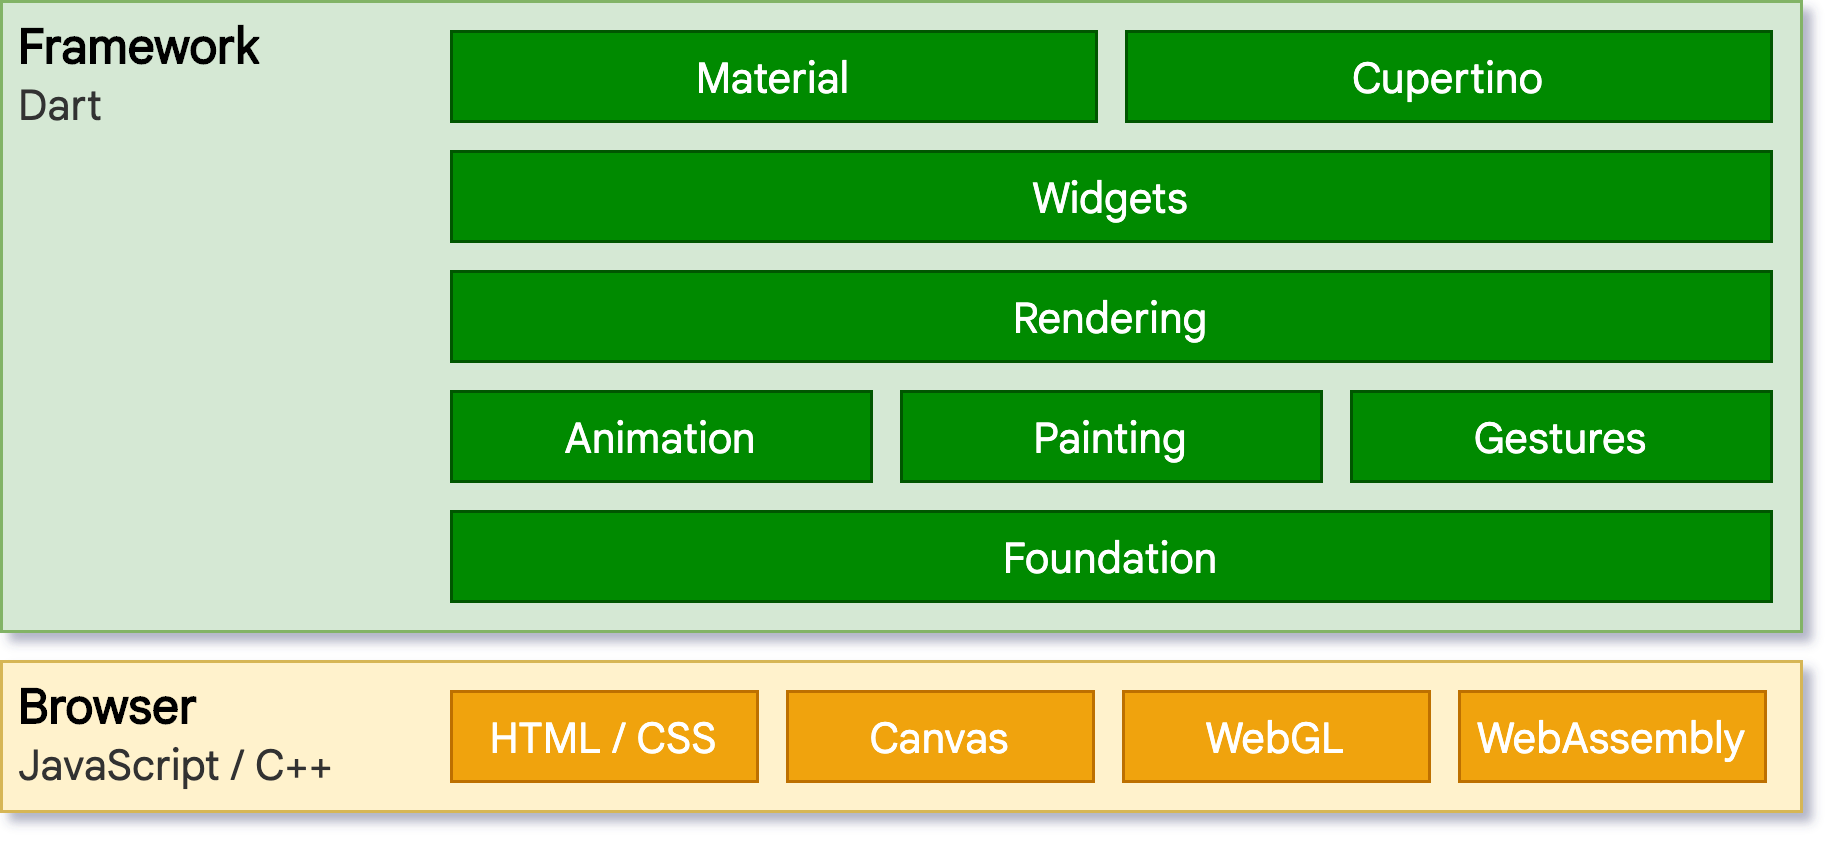
\includegraphics[width=1\linewidth]{assets/design/flutterweb.png}
    \caption{Flutter on Web~\cite{a2022_flutter_architecture}}
    \label{fig:design:flutterweb}
\end{figure}

\pagebreak

Widgets and Composition sections in the~Flutter documentation~\cite{a2022_flutter_architecture} also mention that Flutter uses widgets as building blocks of the~user interface.
Each widgets nests inside its parent, and together they form one hierarchy of widgets.
The~hierarchy of widgets also declares widgets' size, styles, or transformations.
Basic widgets are \mintinline{text}{Collumn} and \mintinline{text}{Row}, for layout of children widgets in a~collumn or a~row; \mintinline{text}{Stack} for stack-based layouts; and \mintinline{text}{Container} as a~generic purpose widget.
Widgets use composition rather than an~extension, and they are usually split into small single-purpose widgets.

The~framework uses two types of widgets: stateful and stateless~\cite{a2022_flutter_architecture}.
\linebreak
If the~widget does not change over time and therefore does not have a~state itself, the~\mintinline{text}{StatelessWidget} widget is used.
If the~widget changes its state, the~\mintinline{text}{StatefulWidget} is used.
Such a~widget is assigned a~unique \mintinline{text}{State}\linebreak{}object that holds the~state of the~widget, and the~widget must call \mintinline{text}{setState()} method each time its state changes and needs to be redrawn.
The~framework responds to the~call to this method and redraws it in the~next cycle.
Separating widgets into stateful and stateless improves application performance by not having to browse and render unchanged widgets.
In addition, thanks to a~separate state and widget, the~framework can support a~hot reload function, which allows the~app to rebuild widgets, i.e., appearance, but maintain the~state of the~respective widgets if they are in the~same place and the~framework can map them.

Whenever it is needed to redraw a~widget, its \mintinline{text}{build()} method is called.
Calling the~\mintinline{text}{build()} method, as mentioned in~\cite{a2022_flutter_architecture}, returns the~subtree of widgets according to which the~UI is rendered.
Because each widget can consist of others, a~tree of all widgets must be made recursively.
During this time, Flutter creates a~tree element that contains an~element for each widget.
\linebreak
The~element represents a~widget instance and represents either\linebreak{}the~element that participates in the~rendering (\mintinline{text}{RenderObjectElement})\linebreak{}or the~element that engages in composing the~hierarchy.
Another tree is created from this tree, a~tree that defines an~abstract model for layout and rendering consisting of the~general \mintinline{text}{RenderObject}.
During the~build phase, Flutter goes through the~\mintinline{text}{RenderObjectElement} in the~element tree and creates a~specific \mintinline{text}{RenderObject} for each.
Flutter traverses the~tree and transmits the~constraints downwards to determine the~layout, while the~descendants transmit their constraints, which must respect the~constraints.
This process can be seen in the~figure~\ref{fig:design:fluttertrees}.

\begin{figure}
    \centering
    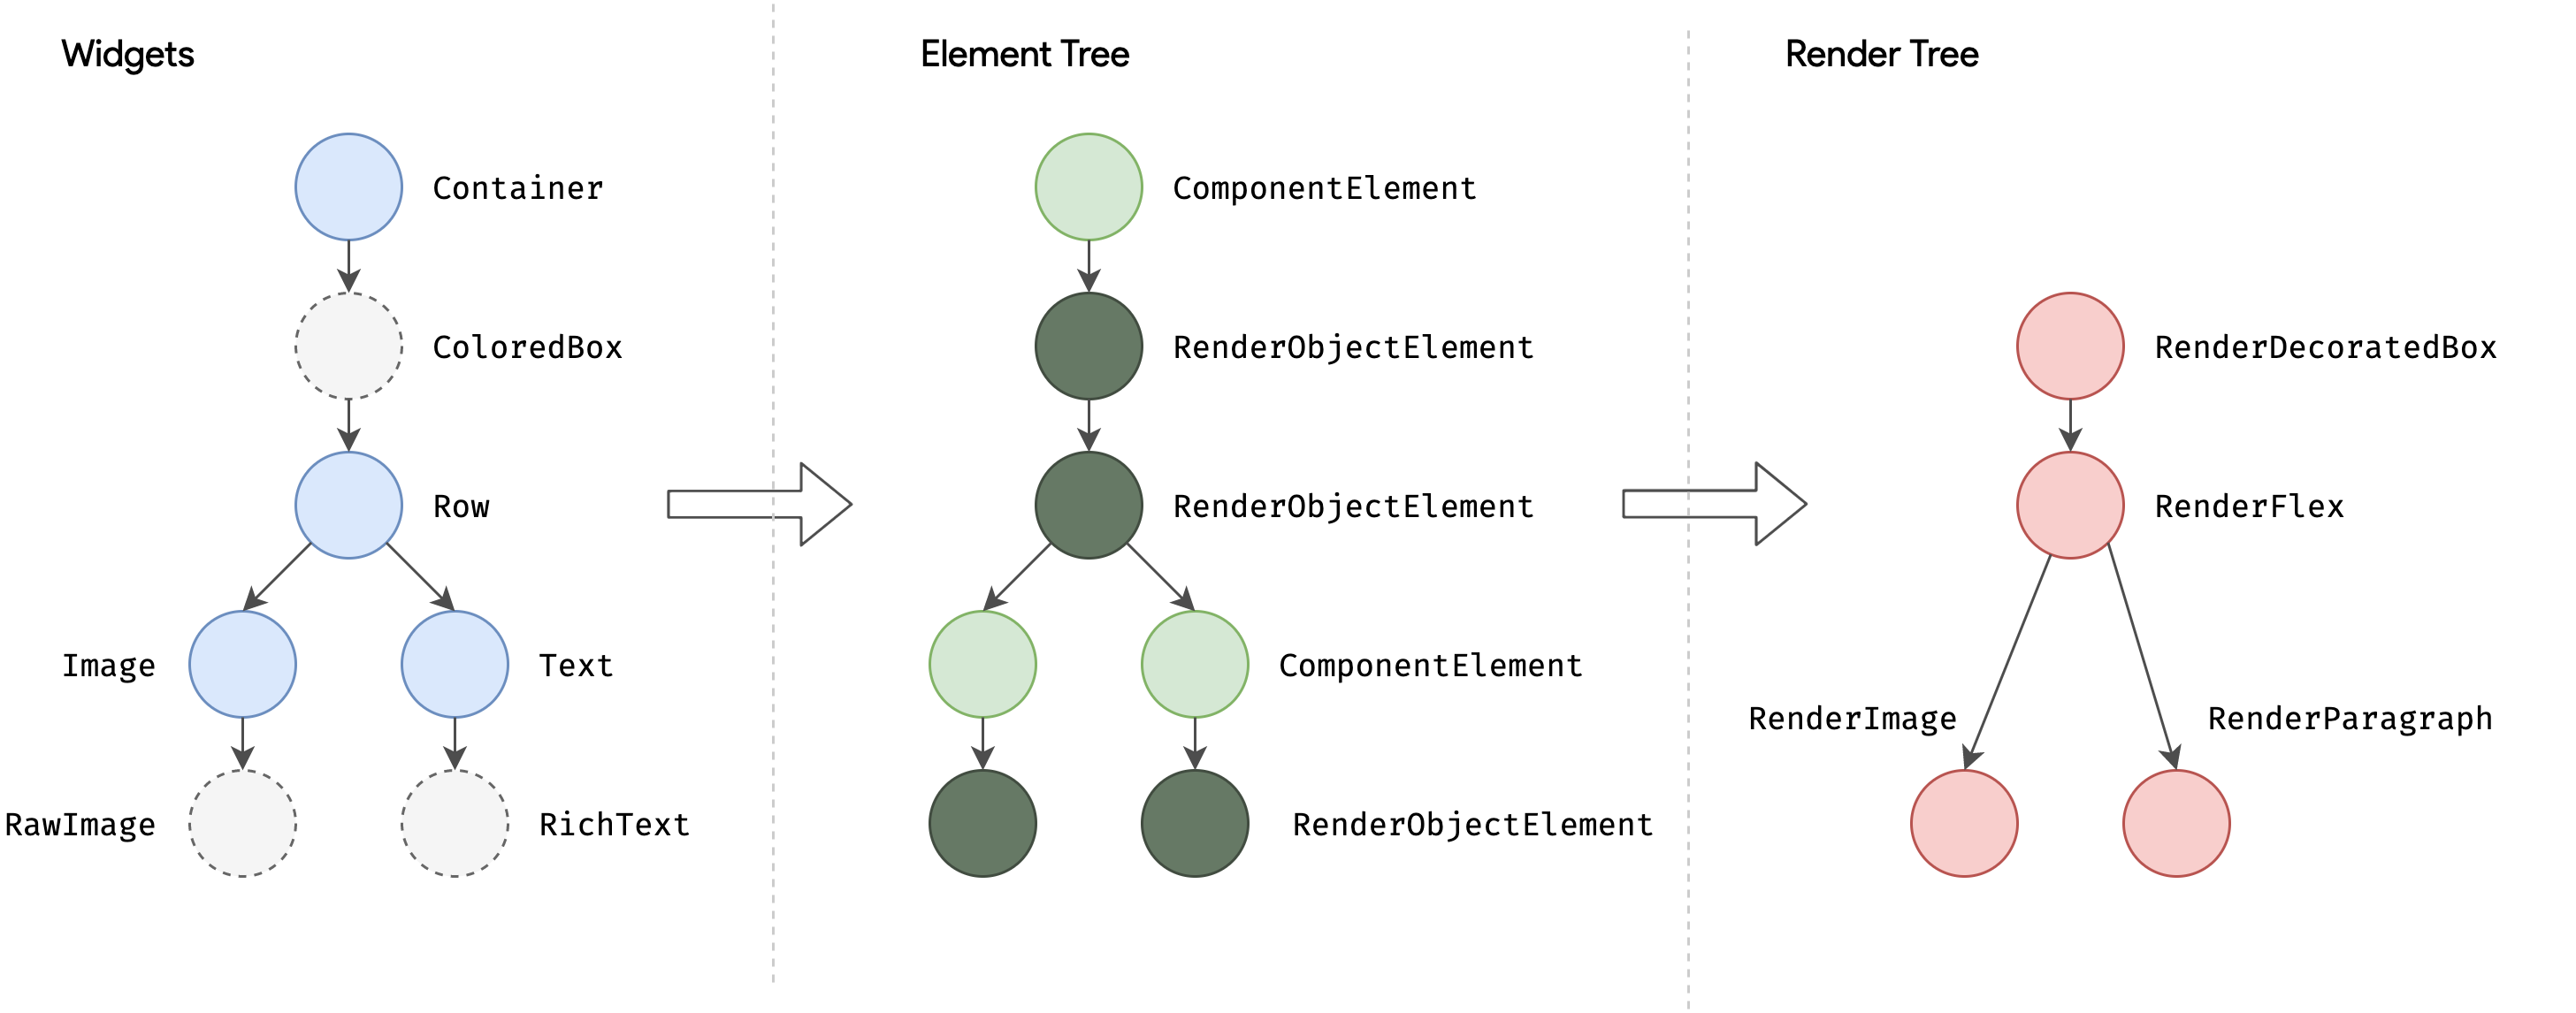
\includegraphics[width=1\linewidth]{assets/design/fluttertrees.png}
    \caption{Flutter Layout and Rendering~\cite{a2022_flutter_architecture}}
    \label{fig:design:fluttertrees}
\end{figure}

As mentioned, Flutter offers many benefits: compilation to native code, being able to compile using AOT and JIT, having a~fast performance, and much more.
It can also build for mobile platforms, desktops, and the~web.
That includes Android, iOS, Windows, Linux, macOS, and web.
Therefore, the~Flutter framework will be used to develop the~game.
With Flutter, the~game can be implemented as a~web version and a~Windows version (with a~Linux and a~macOS versions).
Also, it can be easily extended to mobile to provide an~Android and an~iOS version in the~future.
React Native would also be a~good choice, yet using JavaScript-based technology with its poor static analysis and dealing with other issues coming from the~JavaScript ecosystem is not preferable.
Therefore, Flutter was selected as a~better candidate.

\subsection{Architecture}

As mentioned in chapter~\ref{design:architecture:clean-archiecture}, the~client application should adhere to a~version of the~Clean Architecture.
Its layers should be divided into multiple layers: business contracts, business, data, and presentation.

\begin{figure}
    \centering
    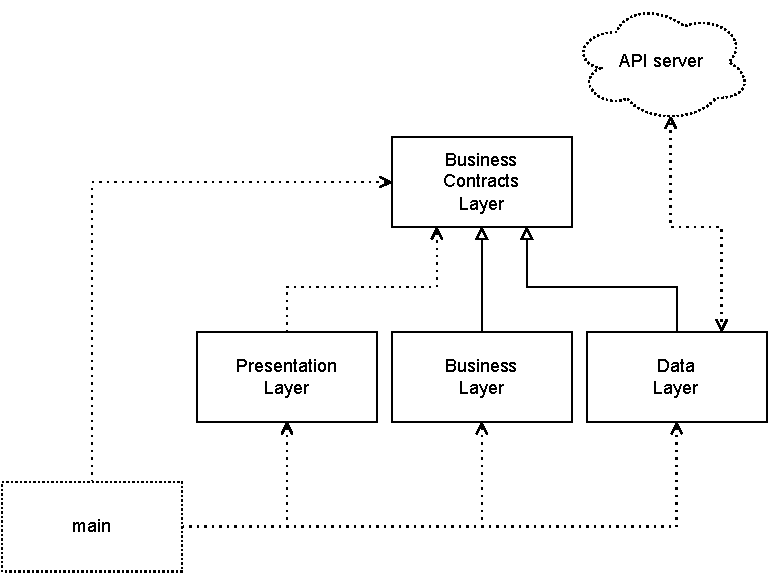
\includegraphics[width=1\linewidth]{assets/design/clientarchitecture.pdf}
    \caption{Client Architecture}
    \label{fig:design:clientarchitecture}
\end{figure}

The~business contracts layer contains entities and all contracts needed for services and repositories.
This layer describes the~interface that other layers use, and its interfaces do not contain any logic other than entities that can have a~simple entity modifying logic.
These layers should be isolated and should not use or know about any other layers.
It also should not use any external packages, especially with some logic.
It might use some external packages that help create interfaces or entities, nothing else.

The~business layer contains contracts implementations from the~business contracts layer, and it implements all services.
Some services might use contracts for repositories, but this layer does not implement those.
The~layer uses repositories' interfaces and gets specific instances as dependencies from constructors.

The~data layer contains implementations from the~business contracts layer, and it implements all repositories.
The~purpose of this layer is to implement repositories that communicate with the~API server.
Repositories are simple workers that process communication with the~external world.

And last but not least, the~presentation layer implements the~UI of the client application.
It uses services' contracts to request specific implementations by the~dependency injection tool registered with services and repositories in the~main method.
The~dependency injection tool provides repositories that are used by the~registered services.

The~main method registers all business contracts layer's interfaces to its dependency injection (DI) container and assigns them with specific implementations from business data layers.
Then it runs the~app.

\pagebreak

As can be seen from the~description and the~figure~\ref{fig:design:clientarchitecture}, the~client architecture follows the~SOLID principles, mainly the~dependency inversion principle. 

\subsection{State Management}

In order for the~client application design to be complete, it is necessary to determine how it will process its state.
That is possible by simple variables and passing up and down from the~widget to the~widget.
As can be seen, this would not be the~most efficient solution, especially since passing data from the~top widget to the~bottom ultimately would require passing data across multiple layers.
For this purpose, developers use state management procedures that allow data to be transferred differently.
Proper design and use of state management will also support the~sustainability and scalability of the~application, which is one of the~non-functional requirements.

Flutter is a~declarative framework~\cite{a2022_flutter_declarative}.
That means the~framework does not use an~imperative method to manage widgets and other framework parts, but rather the~framework expects that state changes, and the~framework then rebuilds and updates the~UI.
In other words, the~user interface is a~function of the~state.
This approach is atypical in many frameworks, such as the~Android SDK, and the~imperative method is often used.
The~declarative principle should also be maintained in state management.
Thanks to the~declarative approach, there is only one way to get to the~desired state, bringing many benefits.
On the~contrary, the~disadvantage of this approach is that it is initially non-intuitive.

According to~\cite{a2022_differentiate}, there can be several types of states in the~software.
And anything that is stored in memory at runtime could be considered a~state.
A better definition of states from an~architectural point of view is \textcquote{a2022_differentiate}{whatever data you need in order to rebuild your UI at any moment in time.}
States are often divided into ephemeral and app states.

An ephemeral state, also often referred to as a~UI state, is a~state that is relevant to only one widget, and only that widget works with it~\cite{a2022_differentiate}.
In this case, there is no need for the~state to be shared in any way with other parts of the application, as this would add unnecessary communication and the~need for more complex logic.
An example of such a~state can be the~current navigation tab.
For an~ephemeral state, it is enough to use the\linebreak{}\mintinline{text}{StatefulWidget} widget and use the~\mintinline{text}{setState()} method to notify the~widget and then redraw it.

In contrast, the~app state, sometimes referred to as the~shared state, is part of several parts of the~application~\cite{a2022_differentiate}.
So this state is trivially not ephemeral.
App state needs more complex management because it is used by multiple parts of the~application, which are often independent and far apart.
The~choice of the~appropriate type of management for such a~state depends on the\linebreak{}complexity of the~application.
An example of an~app state can be the\linebreak{}management of information about a~logged-in user, a~shopping cart in an \mbox{e-shop}, settings, etc.

Whether to use ephemeral or app state may not always be clear.
\linebreak
Ephemeral states can also be used outside the~widget by passing callbacks; however, if a~callback is passed more than one level, it will probably be possible to use another solution.
\textcquote{a2022_differentiate}{The~rule of thumb is: Do whatever is less awkward.}
Some of the~most used state management tools are MobX, Redux, and BLoC.

\subsubsection{MobX}

MobX is a~state management library with three concepts: Observables,\linebreak{}Actions, and Reactions~\cite{a2022_mobxdart}.
This is an~implementation of the~observer \mbox{pattern}.
Concepts are simple in nature and have a~fast learning curve.
According to~\cite{a2022_mobxdart}, the MobX library uses the~following concepts:

\begin{description}
    \item[Observables] Represent states in the~form of any object with data, from numbers to complex objects.
    Data are reactive, which means that each change will notify each observer.
    \item[Actions] Describe changes in the~states of observables. Observables can be changed directly, but actions add semantic meaning, so instead of calling \mintinline{text}{value++} directly, the~\mintinline{text}{increment()} action should be called. The~action triggers a~state change.
    \item[Reactions] Automatically monitor state changes. a~reaction is made immediately after each change.
\end{description}

\subsubsection{Redux}

Redux is a~predictable and centralized state container.
It is one of the~most known libraries on state management.
According to~\cite{brianegan_2021_fluttercommunityreduxdart}, it works with three concepts: Actions, Reducers, and Store:

\begin{description}
    \item[Actions] Represent information sent from the~application to the~store and are its only data source.
    \item[Reducers] Describe how the~application state changed in response to actions.
    Reducers must be pure, which means they must not use non-pure functions and do not mutate the~state; they create a~new copy.
    \item[Store] Represents an~object that holds the~application state.
    It also provides the~current state and sets up the~initial state.
\end{description}

\subsubsection{BLoC}

The~Business Logic Component (BLoC) is not a~library but a~design pattern.
This pattern consists of simple rules that each implementation must follow, leaving specific implementation elements to developers.
According to~\cite{paolosoares_2018_flutter} these design rules are:

\begin{enumerate}
    \item Inputs and outputs are simple
    \mintinline{text}|Stream|/\mintinline{text}|Sink| only.
    \item Dependencies must be injectable and platform agnostic.
    \item No platform branching allowed.
    \item Implementation can be whatever you want
    if you follow the~previous rules.
\end{enumerate}

BLoC also has rules for UI design.
These rules describe the~relationship between the~UI component and the~BLoC component.
According to~\cite{paolosoares_2018_flutter} these rules are:

\begin{enumerate}
    \item Each \textquote*{complex enough} component has a~corresponding BLoC.
    \item Components should send inputs \textquote*{as is}.
    \item Components should show outputs as close as possible to \textquote*{as is}.
    \item All branching should be based on simple BLoC boolean outputs.
\end{enumerate}

This design pattern was created to separate code with logic
from platform-specific dependencies~\cite{paolosoares_2018_flutter}.
In contrast to the~Redux library, the~BLoC pattern works with multiple state stores.

There is a~Bloc library by Alex Angelov for Dart language that implements the~BLoC pattern~\cite{angelov_2022_bloc}.
It tries to implement the~rules described above using the~\mintinline{text}{Stream} and \mintinline{text}{Sink} classes, which allow asynchronous communication.
In addition, this library provides unique Flutter widgets that help listen to changes and rebuild widgets.
This library works with four basic concepts: Events, States, Transitions, Blocs.
In parallel, the~library also provides a~version called Cubit, which works with functions instead of events.
That allows events to be triggered synchronously using functions instead of adding an~event to the~Stream.
Cubit can be easier for smaller applications that can handle more straightforward logic.
According to~\cite{angelov_2022_bloc}, the Bloc library uses the\linebreak{}following concepts:

\pagebreak

\begin{description}
    \item[Events] Represent events in the~form of any object.
    It is the~only input that comes inside the~Bloc.
    \item[States] Represent states in the~form of any object.
    \item[Transitions] Describes the~transition from one state to another, consisting of the~current state, the~next state, and the~triggered event.
    \item[Blocs] Represent classes extending the~Bloc class.
    They accept events, output states, and handle transactions.
    Blocs register event handlers using \mintinline{text}{on<Event>()} methods used in the~constructor.
\end{description}

\subsubsection{Evaluation}

Sending states and callbacks through several levels of widgets is not suitable, so it is not even considered for state management.
Although the~MobX library offers simple concepts and less boilerplate due to code generation, code generation may be slower.
The~Redux and Bloc libraries seem to be similar.
Both work with data asynchronously, but implementations are different.
The~most significant difference is that Redux has only one source of state, while there are multiple in Bloc.
In Redux, only parts of the~states change.
In Bloc, on the~other hand, the~whole state constantly changes.
However, it is small enough and understandable, so it does not cause any problems.
The~Bloc library will be used to develop the~designed game, which will enable an~easy and robust solution thanks to its asynchronous design.
